\documentclass[14pt,a4paper]{extreport}

\usepackage[left=30mm, top=20mm, right=10mm, bottom=20mm]{geometry}
\usepackage{cmap}		
\usepackage[utf8]{inputenc}
\usepackage[english, russian]{babel}
\usepackage{framed}
\usepackage{amsmath}
\usepackage{graphicx}
\usepackage{wrapfig}
\usepackage{listings}
\usepackage{color}
\usepackage{verbatim}
\usepackage{indentfirst}
\usepackage{textcomp}
\usepackage{titlesec}
\usepackage{alltt}
\usepackage{float}
\usepackage{cite}
\usepackage{url}
%%%%%%%%%%%%%%%%%%%%%%%%%%%%%%%%%%%%%%%%%%%%%%%%%%%%%%%%%%%%%%%%%%%%%%%%

\titleformat{\chapter}[display]
    {\filcenter\large\bfseries}
    {\MakeUppercase{\chaptertitlename} \thechapter}
    {8pt}
    {\bfseries}{}
\titleformat{\section}
    {\normalsize\bfseries}
    {\thesection}
    {1em}{}
\titleformat{\subsection}
    {\normalsize\bfseries}
    {\thesubsection}
    {1em}{}

%% Настройка вертикальных и горизонтальных отступов
\titlespacing*{\chapter}{0pt}{-30pt}{8pt}
\titlespacing*{\section}{\parindent}{*4}{*4}
\titlespacing*{\subsection}{\parindent}{*4}{*4}

%% Отступ от левого края
\oddsidemargin=0pt 

\lstdefinestyle{customc}{belowcaptionskip=1\baselineskip,breaklines=true,frame=L,xleftmargin=\parindent,  language=C, showstringspaces=false, basicstyle=\footnotesize\ttfamily,keywordstyle=\bfseries\color{green!40!black},  commentstyle=\itshape\color{purple!40!black}, identifierstyle=\color{blue}, stringstyle=\color{orange},numbers=left,numbersep=12pt, numberstyle=\small\color{mygray},}
\lstset{escapechar=@,style=customc}

\newcommand{\HRule}{\rule{\linewidth}{0.5mm}}

\begin{document}

%% Титульный
%%%%%%%%%%%%%%%%%%%%%%%%%%%%%%%%%%%%%%%%%%%%%%%%%%%%%%%%%%%%%%%%%%%%%%%%
\begin{titlepage}
\begin{center}


{\normalsize 
Федеральное государственное автономное образовательное учреждение высшего образования 
\\Санкт-Петербургский национальный исследовательский университет 
\\информационных технологий, механики и оптики}

\vspace{1.5cm}

\vspace{0.5cm}
\large Факультет систем управления и робототехники
% Upper part of the page. The '~' is needed because \\
% only works if a paragraph has started.
%\includegraphics[width=0.18\textwidth]{img/logo.png}~\\[1cm]
\vspace{2cm}

\large Курсовой проект
\\ Вариант №2

по дисциплине <<Программирование систем управления>>

{ \large \bfseries <<Моделирование системы управления>>\\[0.4cm] }

% Author and supervisor
\noindent

\begin{flushright} \normalsize
\emph{Выполнили:}\\
Студент группы R41332\\
Волков \textsc{А.~А.}\\
% Щербаков \textsc{П.~В.}\\

\emph{Проверил:} \\
Томашевич \textsc{С.~И.}
\end{flushright}

\vfill

% Bottom of the page
{\normalsize Санк-Петербург, 2019 г.}

\end{center}
\end{titlepage}

%%%%%%%%%%%%%%%%%%%%%%%%%%%%%%%%%%%%%%%%%%%%%%%%%%%%%%%%%%%%%%%%%%%%%%%%

%% Оглавление
%%%%%%%%%%%%%%%%%%%%%%%%%%%%%%%%%%%%%%%%%%%%%%%%%%%%%%%%%%%%%%%%%%%%%%%%
\newpage
\tableofcontents
%%%%%%%%%%%%%%%%%%%%%%%%%%%%%%%%%%%%%%%%%%%%%%%%%%%%%%%%%%%%%%%%%%%%%%%%

%% Задание
%%%%%%%%%%%%%%%%%%%%%%%%%%%%%%%%%%%%%%%%%%%%%%%%%%%%%%%%%%%%%%%%%%%%%%%%
\chapter*{Задание}
\addcontentsline{toc}{chapter}{Задание}

\begin{enumerate}
\item
Реализовать класс интегратора в .cpp и .h файлах.
    
\item 
Привести задающее воздействие в виде модели с использованием интегратором.
    
\item 
Дисретизировать полученные модели задающего воздействия 
и объекта управления с шагами дискретизации 5, 50, 100 Гц.

\item
Программно реализовать отдельными классами четыре случая объектов 
(непрерывный и три дискретных). Для дискретных случаев сделать 
реализацию с использованием разностных уравнений.
\begin{equation} 
    x_{k+1} = A \cdot x_k
\end{equation}
То есть интегратор заменяется на элемент памяти.

\item 
Добавить реализованные классы в предоставленную программу для \\ QtCreator.

\item
Поочередно провести сравнение поведений реализованных непрерывв-
ных моделей с дискретными моделями с соответствующими шагами
дискретизации. Шаг дискретизации меняется в предоставленной про-
грамме. В результате должно получиться три пары сравнений.

\item 
В предоставленной программе QtCreator настроить последовательный
порт (qSerialPort) на скорость 115200 бод, формат 8N1.

\item 
Закодировать с помощью метода COBS значения, полученные с выхода
объекта в следующем формате:
{[0x0A 0xXX 0xXX 0xXX 0xXX 0xCR]}, где 0xXX – байты полученного 
числа с плавающей точкой (float) в
обратном порядке, а 0xCR – проверочная сумма, равная сумме всех
остальных байт сообщения, вычтенной из 0xFF.

\end{enumerate}
%%%%%%%%%%%%%%%%%%%%%%%%%%%%%%%%%%%%%%%%%%%%%%%%%%%%%%%%%%%%%%%%%%%%%%%%

%% Исходные данные
%%%%%%%%%%%%%%%%%%%%%%%%%%%%%%%%%%%%%%%%%%%%%%%%%%%%%%%%%%%%%%%%%%%%%%%%
\newpage
\chapter*{Исходные данные}
\addcontentsline{toc}{chapter}{Исходные данные}

Входной сигнал задается в следующем виде:
\begin{equation}
    u(t) = 3 \cdot  cos(0.1 \cdot t + 1)
\end{equation}

Система представлена в виде Вход-Состояние-Выход. Матрицы A, B, C выглядят следующим образом:
\begin{equation}
    A = 
    \begin{bmatrix} 
        0 & 1 & 0 \\ 
        0 & 0 & 1 \\
        -1.5 & -5 & -2
    \end{bmatrix}
\end{equation}

\begin{equation}
    B = 
    \begin{bmatrix} 
        0 \\ 
        0 \\
        1
    \end{bmatrix}
\end{equation}

\begin{equation}
    C = 
    \begin{bmatrix} 
        0.5 & 0 & 0
    \end{bmatrix}
\end{equation}

Расчет выходного сигнала проходит по следующим формулам:
\begin{equation}
\dot x = A \cdot x + B \cdot u(t)
\end{equation}

\begin{equation}
y = C \cdot x
\end{equation}
%%%%%%%%%%%%%%%%%%%%%%%%%%%%%%%%%%%%%%%%%%%%%%%%%%%%%%%%%%%%%%%%%%%%%%%%

%% Ход работы
%%%%%%%%%%%%%%%%%%%%%%%%%%%%%%%%%%%%%%%%%%%%%%%%%%%%%%%%%%%%%%%%%%%%%%%%
\chapter*{Ход работы}
\addcontentsline{toc}{chapter}{Ход работы}
Исходный код программы представлен в приложении А. 

Непрерывная система отличается от дискретной отличается способом 
расчета вектора состояния и параметрами системы. Переходные процессы для дискретной и непрерывной системы отличаются 
только в случае очень большого шага дискретизации.

Переходной процесс непрерывной системы 
представлен на рис.\ref{fig:contin}.
\begin{figure}[H]
    \centering
    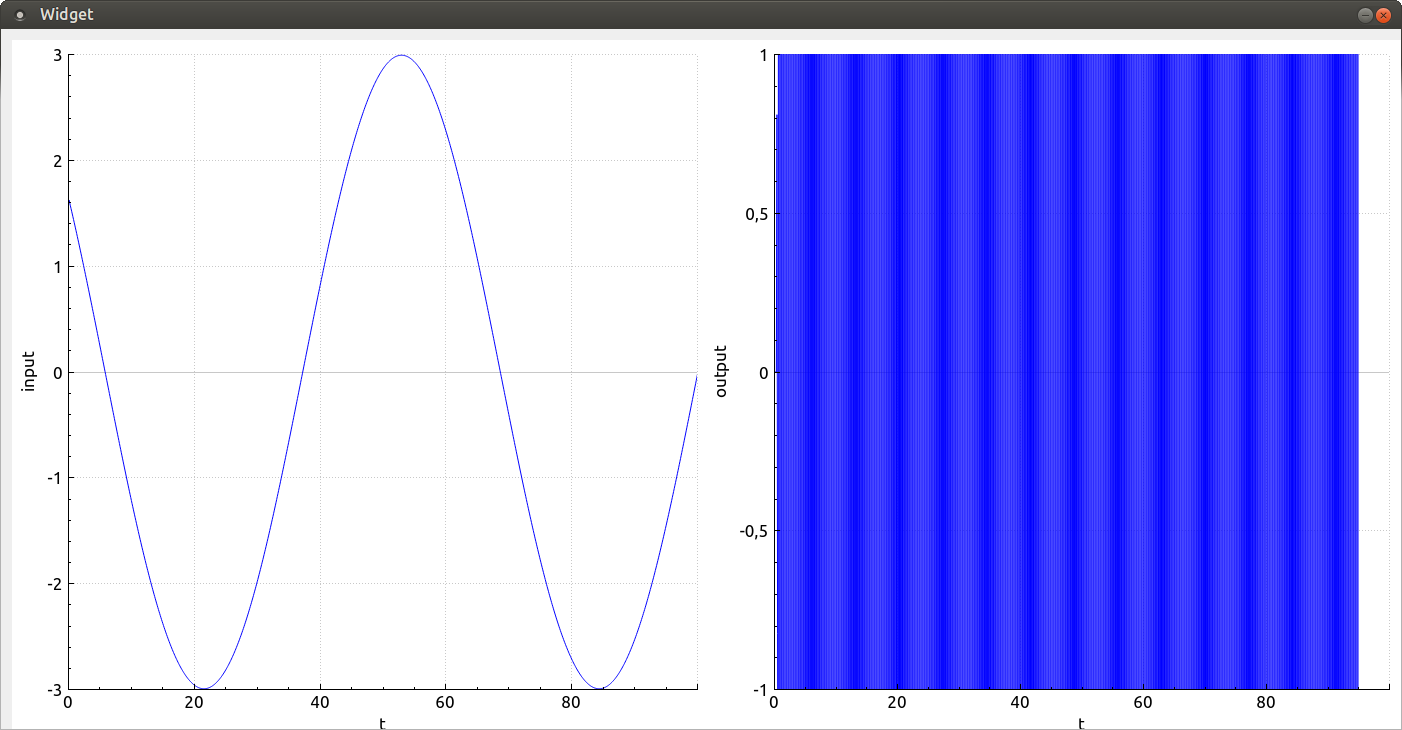
\includegraphics[width=160mm]{img/cont.png}
    \caption{Переходной процесс непрерывной системы}
    \label{fig:contin}
\end{figure}

Переходной процесс дискретной системы с шагом дискретизации 
5 Гц представлен на рис.\ref{fig:discrete5}.
\begin{figure}[H]
    \centering
    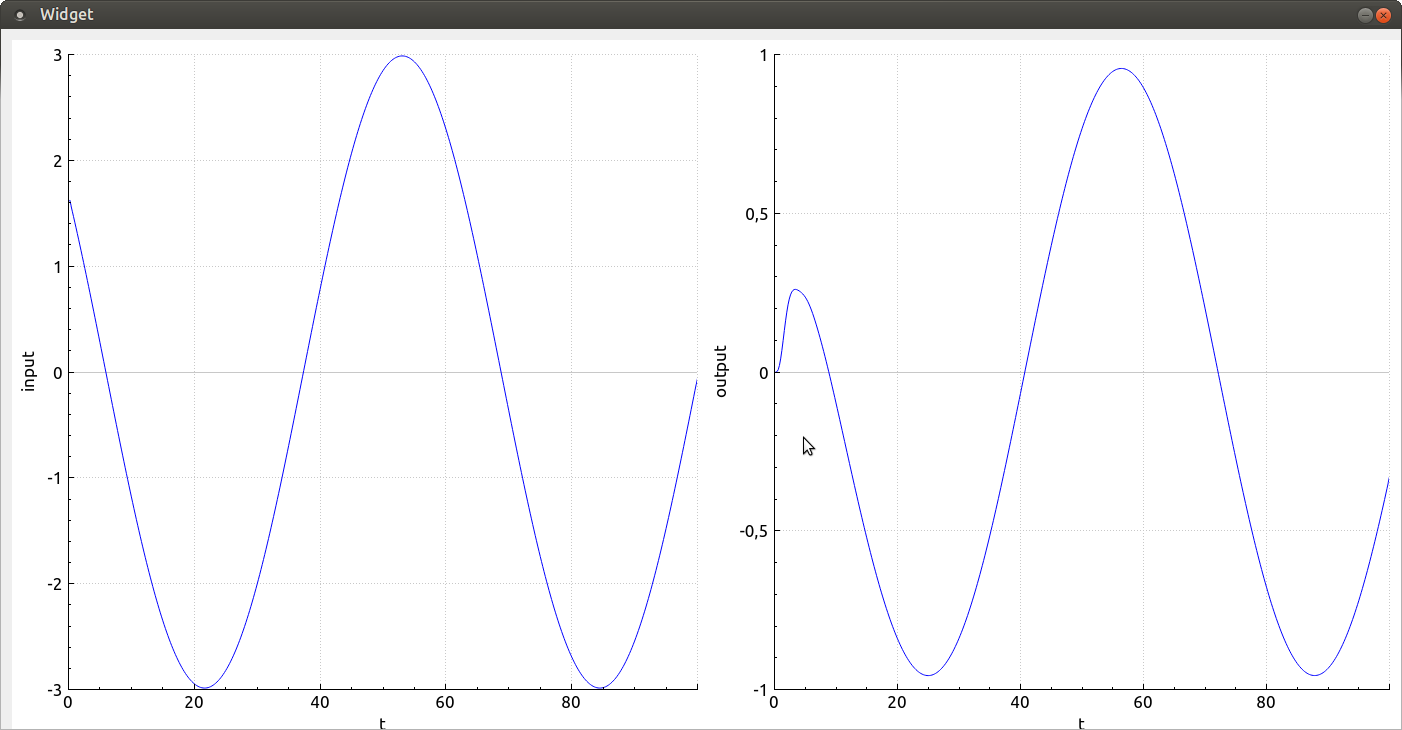
\includegraphics[width=160mm]{img/5hz.png}
    \caption{Переходной процесс дискретной системы 
    с шагом дискретизации 5 Гц}
    \label{fig:discrete5}
\end{figure}

Переходной процесс дискретной системы с шагом дискретизации 
50 Гц представлен на рис.\ref{fig:discrete50}.

\begin{figure}[H]
    \centering
    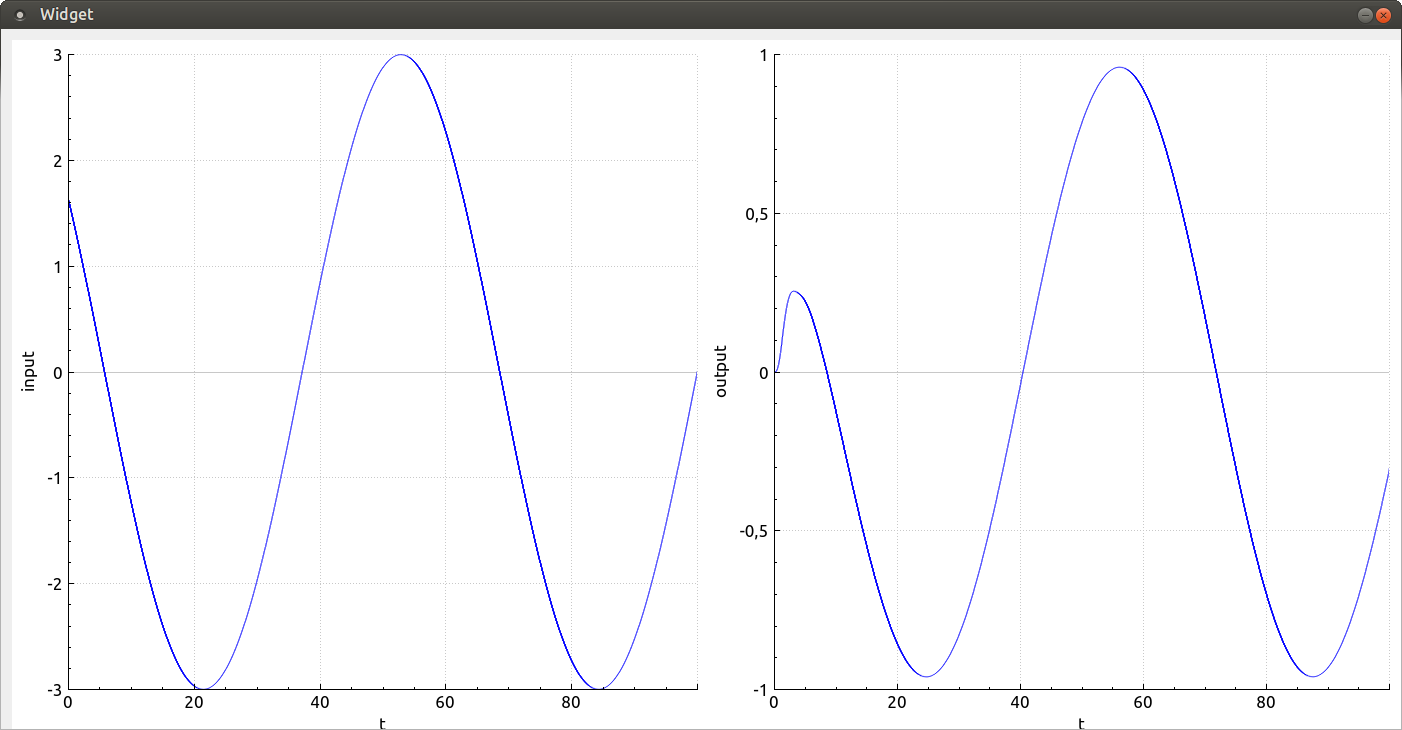
\includegraphics[width=160mm]{img/50hz.png}
    \caption{Переходной процесс дискретной системы 
    с шагом дискретизации 50 Гц}
    \label{fig:discrete50}
\end{figure}

Переходной процесс дискретной системы с шагом дискретизации 
100 Гц представлен на рис.\ref{fig:discrete100}.

\begin{figure}[H]
    \centering
    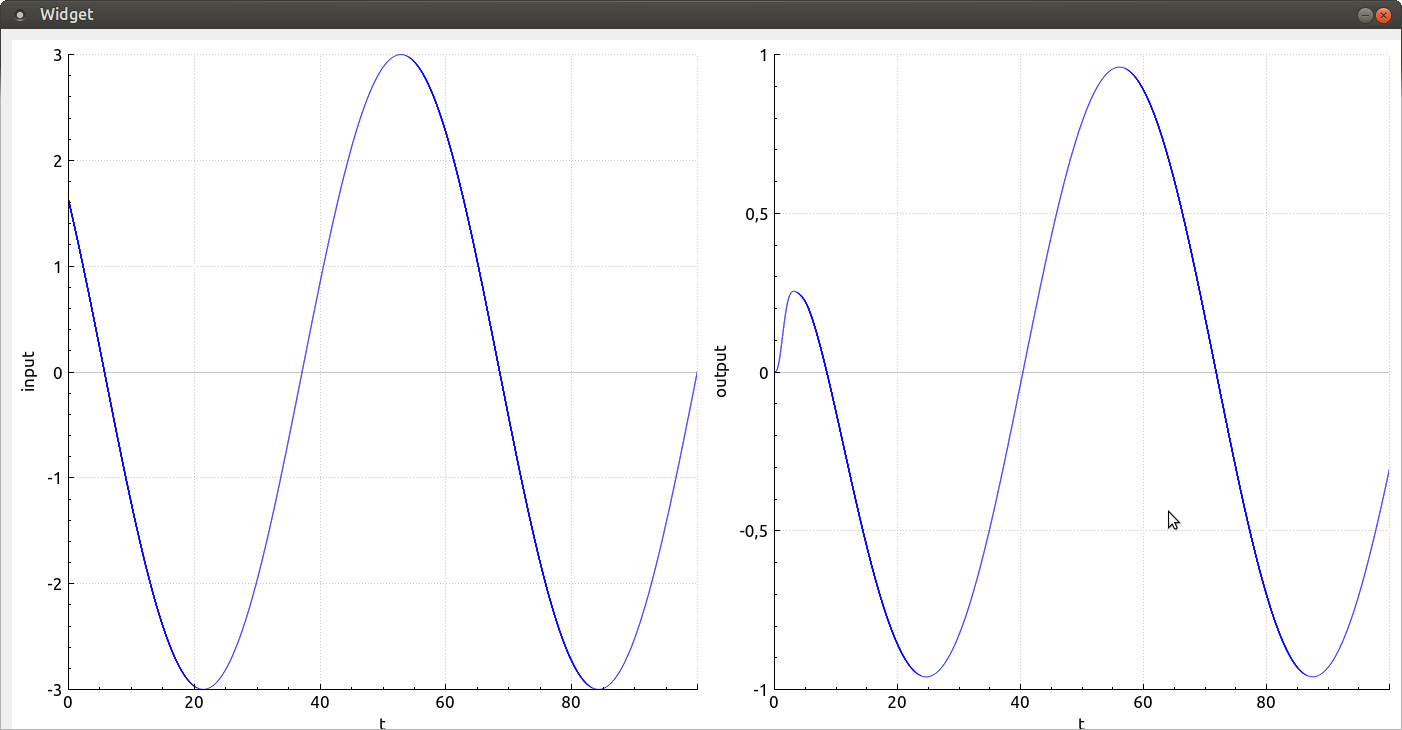
\includegraphics[width=160mm]{img/100hz.png}
    \caption{Переходной процесс дискретной системы 
    с шагом дискретизации 100 Гц}
    \label{fig:discrete100}
\end{figure}

Для проверки работы UART был эмулирован терминал OS Linux, в который было отправлено тестовое значение 
42.0 используя заданные параметры передачи данных. 
Результат отправки представлен на рис.\ref{fig:uart}.
\begin{figure}[H]
    \centering
    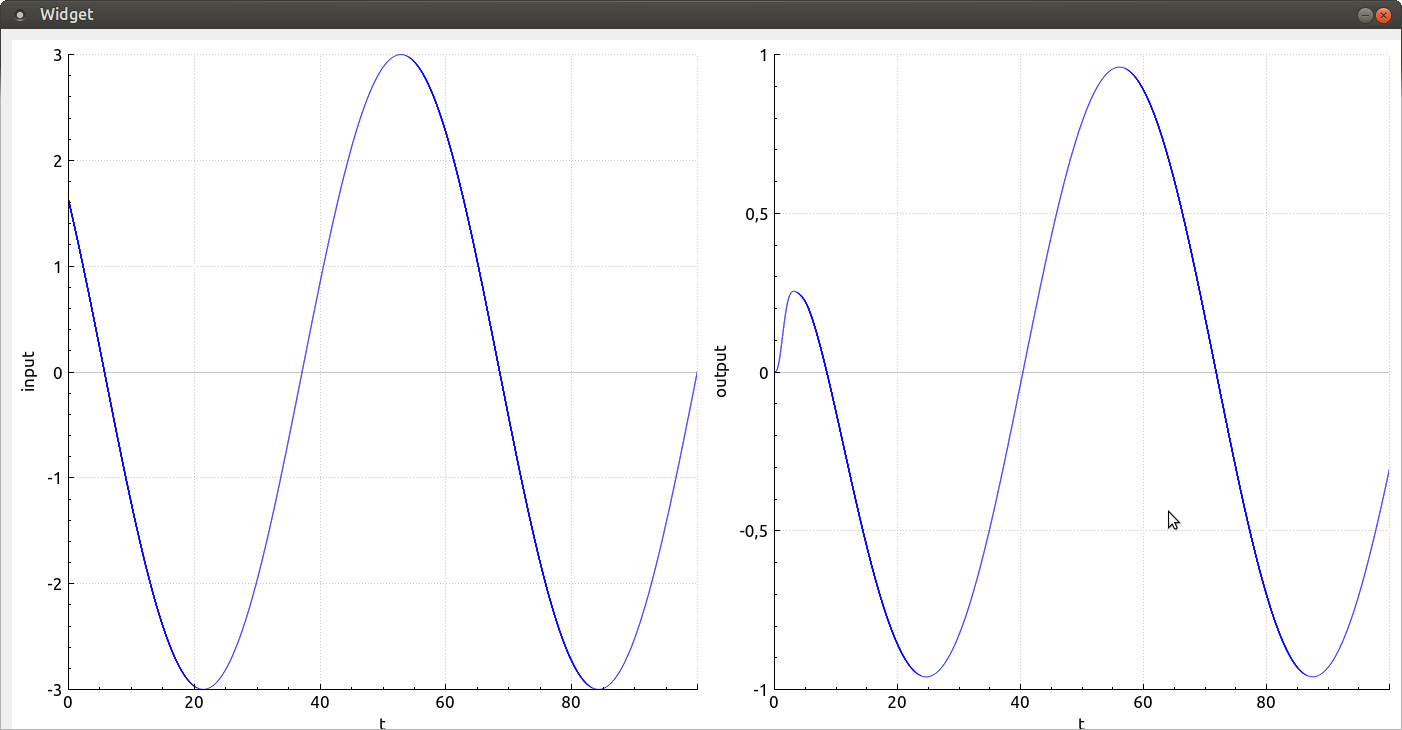
\includegraphics[width=160mm]{img/100hz.png}
    \caption{Отправка сигнала по UART}
    \label{fig:uart}
\end{figure}

Кодировка сигнала происходит с помощью стороннего заголовочного файла. 
Результат кодировки сигнала 42.0 представлен на рис.\ref{fig:cobs}.
\begin{figure}[H]
    \centering
    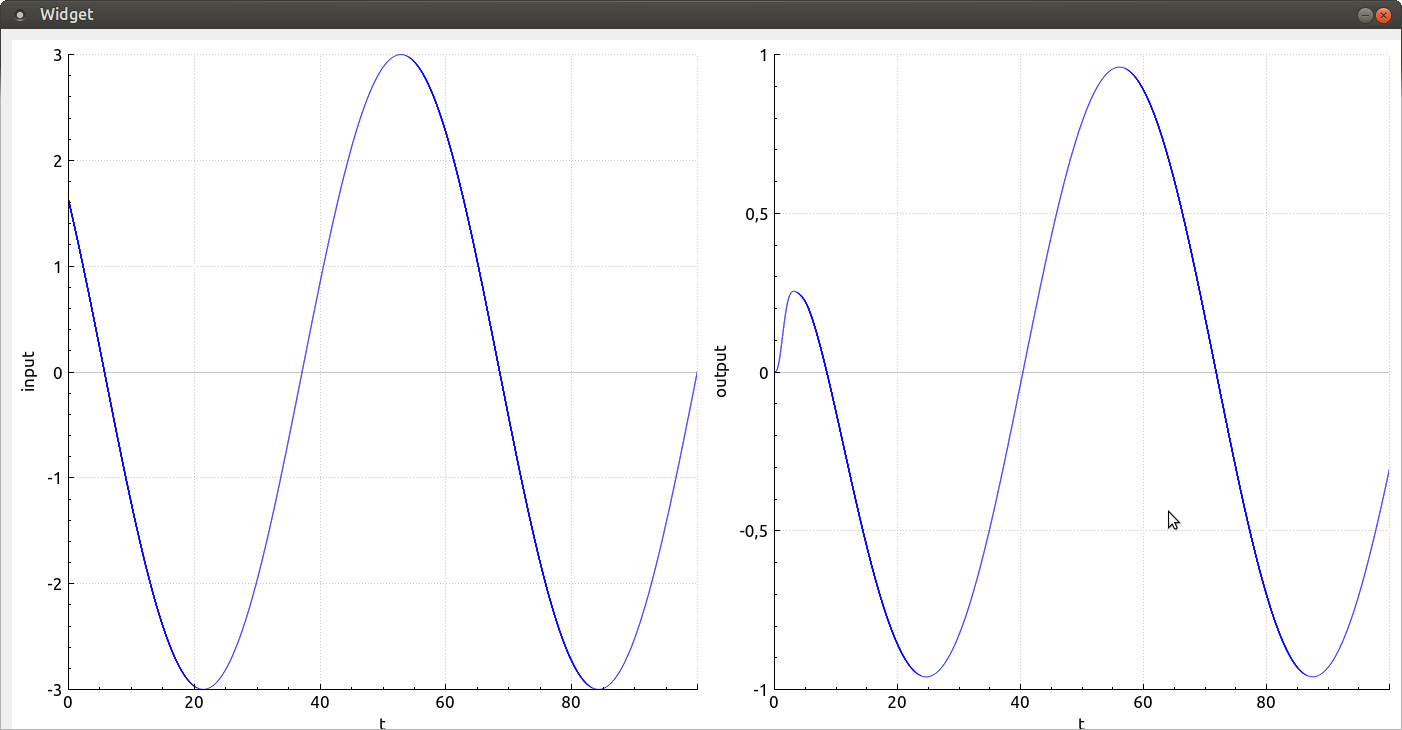
\includegraphics[width=160mm]{img/100hz.png}
    \caption{Отправка зашифрованного сигнала}
    \label{fig:cobs}
\end{figure}
%%%%%%%%%%%%%%%%%%%%%%%%%%%%%%%%%%%%%%%%%%%%%%%%%%%%%%%%%%%%%%%%%%%%%%%%

%% Приложение А. Исходный код программы
%%%%%%%%%%%%%%%%%%%%%%%%%%%%%%%%%%%%%%%%%%%%%%%%%%%%%%%%%%%%%%%%%%%%%%%%
\newpage
\chapter*{Приложение А. Исходный код программы}
\addcontentsline{toc}{chapter}{Приложение А. Исходный код программы}

\textbf{Файл model.h}
\begin{alltt}
    \verbatiminput{./../src/qt/model/model.h}
\end{alltt}

\textbf{Файл model.cpp}
\begin{alltt}
    \verbatiminput{./../src/qt/model/model.cpp}
\end{alltt}

\textbf{Файл integrator.h}
\begin{alltt}
    \verbatiminput{./../src/qt/model/integrator.h}
\end{alltt}

\textbf{Файл integrator.cpp}
\begin{alltt}
    \verbatiminput{./../src/qt/model/integrator.cpp}
\end{alltt}

\textbf{Файл matrix.h}
\begin{alltt}
    \verbatiminput{./../src/qt/model/matrix.h}
\end{alltt}

\textbf{Файл matrix.cpp}
\begin{alltt}
    \verbatiminput{./../src/qt/model/matrix.cpp}
\end{alltt}

\textbf{Файл main.cpp}
\begin{alltt}
    \verbatiminput{./../src/qt/main.cpp}
\end{alltt}

\textbf{Файл widget.h}
\begin{alltt}
    \verbatiminput{./../src/qt/view/widget.h}
\end{alltt}

\textbf{Файл widget.cpp}
\begin{alltt}
    \verbatiminput{./../src/qt/view/widget.cpp}
\end{alltt}

\textbf{Файл cobs.h}
\begin{alltt}
    \verbatiminput{./../src/qt/model/cobs.h}
\end{alltt}
%%%%%%%%%%%%%%%%%%%%%%%%%%%%%%%%%%%%%%%%%%%%%%%%%%%%%%%%%%%%%%%%%%%%%%%%

\end{document}
